To specify some rules about how a program in Lattice should be composed, we have written the following context-free grammar, using Extended Backus-Naur form.
This grammar can then be used to build a parser and recognize valid Lattice programs and their structure.

\subsubsection*{Global composition of a program}

A program in Lattice would be a sequence of statements and function definitions.

\begin{align*}
    \mathit{Start} \rightarrow \{ \mathit{FunctionDef} \mid \mathit{Statement} \}
\end{align*}
\captionedgrammar{Description of the global structure of a program}

Statements can be variable declarations, variable assignments, graph manipulation (i.e.\ opening a graph context to do operations), print statements, blocks of code in an if-else control structure or a while loop, or a return statement.

\begin{align*}
    \omit $\mathit{Statement}$ \hfil& \rightarrow \mathit{VarDecl} \\
    & \mid \mathit{VarAssignOrGraphManipOrAddRel} \\
    & \mid \mathit{PrintStatement} \\
    & \mid \mathit{IfBlock} \\
    & \mid \mathit{WhileBlock} \\
    & \mid \mathit{ReturnStatement} \\
    & \mid \mathit{AddRef} \\
    & \mid \mathit{AddClone}
\end{align*}
\captionedgrammar{Description of the different kind of statements}

\subsubsection*{Variable declaration}

A variable is declared by writing its type followed by its name.
After the variable declarations the statement can end with a semicolon or there can be a value assigned to the variable or a graph context can be opened.

There need to be a global production rule for variable assignment, graph manipulation and relation statements because all three of those statements start with a variable identifier so having the rules be fully separated would mean that the grammar isn't LL(1).
Once the variable for which we are writing the statement is specified, the rest of the statement can either correspond to an assignment, a block of code in a graph context or a relation statement.

\begin{align*}
    \omit $\mathit{VarDecl}$ \hfil& \rightarrow \mathit{Type} \: \text{varId} \: \mathit{VarDeclTail} \\
    \omit $\mathit{VarDeclTail}$ \hfil & \rightarrow \mathit{TailVarAssignOrGraphManip} \\
    & \mid \text{semicolon} \\
    \omit $\mathit{VarAssignOrGraphManip}$\hfil & \rightarrow \text{varId} \: \mathit{TailVarAssignOrGraphManip} \\
    \omit $\mathit{TailVarAssignOrGraphManip}$ & \rightarrow \mathit{TailVarAssign} \\
    & \mid  \mathit{TailGraphManip}\ \\
    \omit $\mathit{Type}$ \hfil & \rightarrow \text{typeString} \\
    & \mid \text{typeFloat} \\
    & \mid \text{typeBool} \\
    & \mid \text{typeInt}\\
    & \mid \text{typeGraph}
\end{align*}
\captionedgrammar{Rules for variable declaration}

\begin{figure}[H]
    \centering
    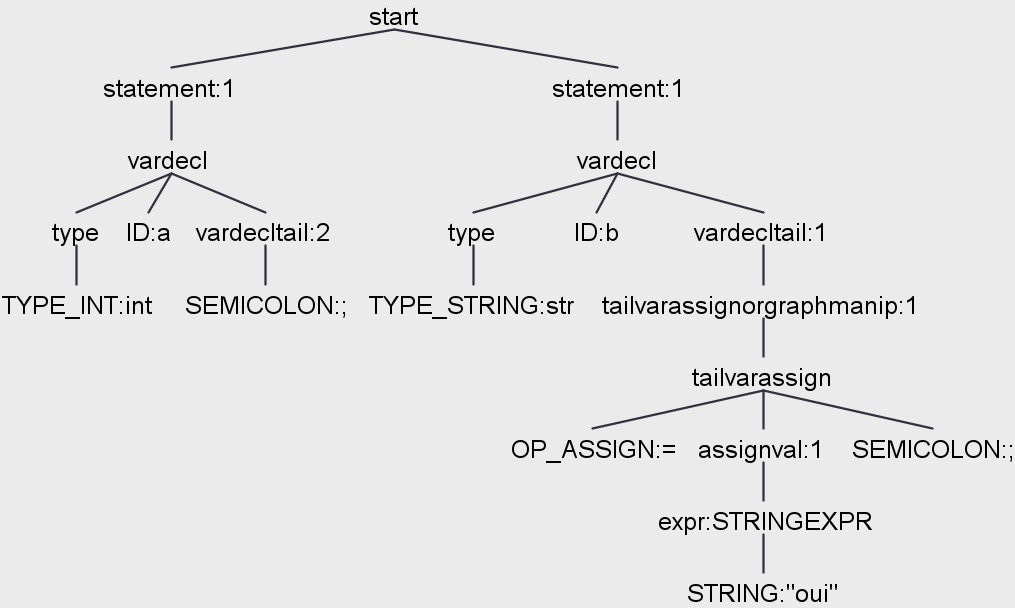
\includegraphics[height = 5cm]{figures/parse_trees/parseTree_varDecl}
    \caption{The parse tree for the statements \texttt{int a;
    str b = "oui";}}
    \label{fig:parseTree_varDecl}
\end{figure}

\subsubsection*{Variable assignment and arithmetic expressions}
To assign a value to a variable, the variable name needs to be followed by the assignment operator and then the assigned value, which can be a string, a boolean value, an arithmetic expression with variables, numbers and function calls or simply a function call, a number or another variable.

\begin{align*}
    \omit $\mathit{TailVarAssign}$ \hfil & \rightarrow \text{opAssign} \: \mathit{AssignVal} \: \text{semicolon} \\
    \omit $\mathit{AssignVal}$ \hfil & \rightarrow \text{string} \\
    & \mid \mathit{Expr} \\
    & \mid \mathit{BoolVal}\\
    \omit $\mathit{Expr}$ \hfil & \rightarrow \text{opSub} \: \mathit{Expr} \\
    & \mid \mathit{Expr} \: \mathit{MulOp} \: \mathit{Expr} \\
    & \mid \mathit{Expr} \: \mathit{AddOp} \: \mathit{Expr} \\
    & \mid \text{leftParen}\: \mathit{Expr} \: \text{rightParen} \\
    & \mid \mathit{Number} \\
    & \mid \text{varId} \\
    & \mid \mathit{FuncCall} \\
    & \mid \text{KeywordFmap} \: \text{varId} \: \text{varId} \\
    \omit $\mathit{BoolVal}$ \hfil & \rightarrow \text{keywordTrue} \\
    & \mid \text{keywordFalse} \\
    \omit $\mathit{Number}$ \hfil & \rightarrow \text{integer} \\
    & \mid \text{floatLit} \\
    \omit $\mathit{AddOp}$ \hfil & \rightarrow \text{opAdd} \\
    & \mid \text{opSub} \\
    \omit $\mathit{MulOp}$ \hfil & \rightarrow \text{opMult} \\
    & \mid \text{opDiv} \\
    & \mid \text{opRem}
\end{align*}
\captionedgrammar{Rules for variable assignment and arithmetic expressions}

This definition of the grammar has a lot of rules but doesn't allow the precedence of arithmetic operations to be handled during the building of the parse tree and makes the grammar ambiguous.
However, those rules allow us to have the desired behavior when we use the tool we have chosen for the implementation (\ref{TODO}).

\begin{figure}[H]
    \centering
    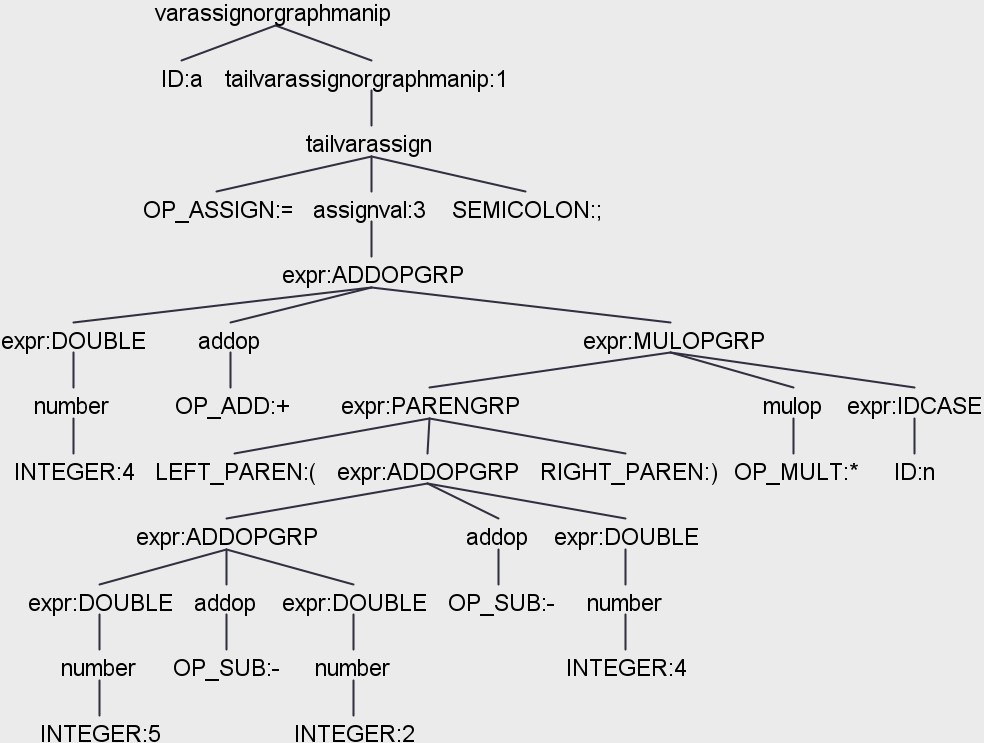
\includegraphics[height = 8cm]{figures/parse_trees/parseTree_varAssign}
    \caption{The parse tree for a variable assignment :  \texttt{a = 4 + (5-2-4)*n;} \\The tool used handled the operation precedence.}
    \label{fig:parseTree_varAssign}
\end{figure}

\subsubsection*{Graph Manipulation}

After having specified the graph context in which we want to work, we can then write the statements to do in this context.
Those might be graph-specific operations such as referencing or cloning a variable using the dedicated keywords, or adding a relation between two variables.

\begin{align*}
    \omit $\mathit{TailGraphManip}$ \hfil &\rightarrow \text{leftBrace} \: \{ \mathit{Statement} \}  \: \text{rightBrace} \\
    \omit $\mathit{AddRel}$ \hfil & \rightarrow \text{varId opRelLeft} \: \mathit{Number} \: \text{comma string opRelRight varId} \\
    \omit $\mathit{AddClone}$ \hfil & \rightarrow \text{keywordClone varId semicolon} \\
    \omit $\mathit{AddRef}$ \hfil & \rightarrow \text{keywordRef varId semicolon}
\end{align*}
\captionedgrammar{Rules regarding graph contexts}

\begin{figure}[H]
    \centering
    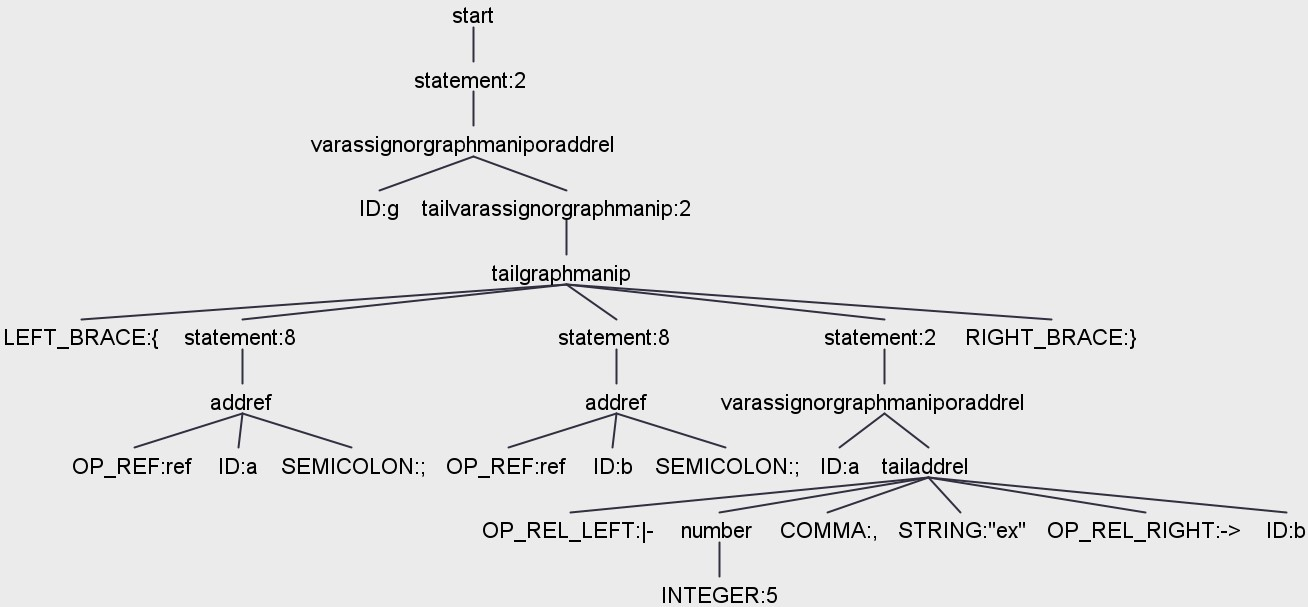
\includegraphics[height = 3.5cm]{figures/parse_trees/parseTree_graphManip}
    \caption{The parse tree for some simple graph operations. The code parsed is \texttt{g\{
        ref a;
        ref b;
        a |-5, "ex" -> b\} }}
    \label{fig:parseTree_graphManip}
\end{figure}

\subsubsection*{Print statement}

The print function is quite minimalist and can only be used for strings and variables, using the keyword $\texttt{print}$.

\begin{align*}
    \mathit{PrintStatement} \rightarrow \text{keywordPrint} \: (\text{varID} \mid \text{string}) \: \text{semicolon}
\end{align*}
\captionedgrammar{Structure of a print statement}

\subsubsection*{If-else statement}

The if-else statement structure is quite classic.
After the \texttt{if} keyword, a boolean expression is specified between parenthesis and then the block of code to execute is written between curly brackets.
The following else clause is optional.

\begin{lstlisting}[caption={test},captionpos=b, label={lst:teststuff}]
    IfBlock
\end{lstlisting}

Since the boolean expression and the arithmetic expression are different, writing an arithmetic expression as the condition of an $\texttt{if}$ statement is a syntax error, not a type error that would be found by the type checker or a semantic error despite what some people might expect.
This distinction also causes our grammar to be bigger complicating the implementation part.
We still made the choice to write our grammar that way because the tool we use gives this grammar some redeeming qualities (\ref{TODO} (future ref))

\begin{figure}[H]
    \centering
    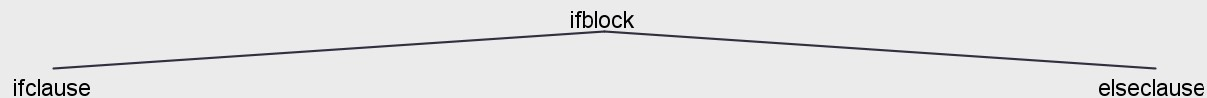
\includegraphics[height = 1cm]{figures/parse_trees/parseTree_ifblock}
    \caption{Top of the parse tree for the following if statement : \texttt{if(c)\{
        a = 5;\}
        else \{
            b = 3;\}}}
    \label{fig:parseTree_ifblock}
\end{figure}

\begin{figure}[H]
    \centering
    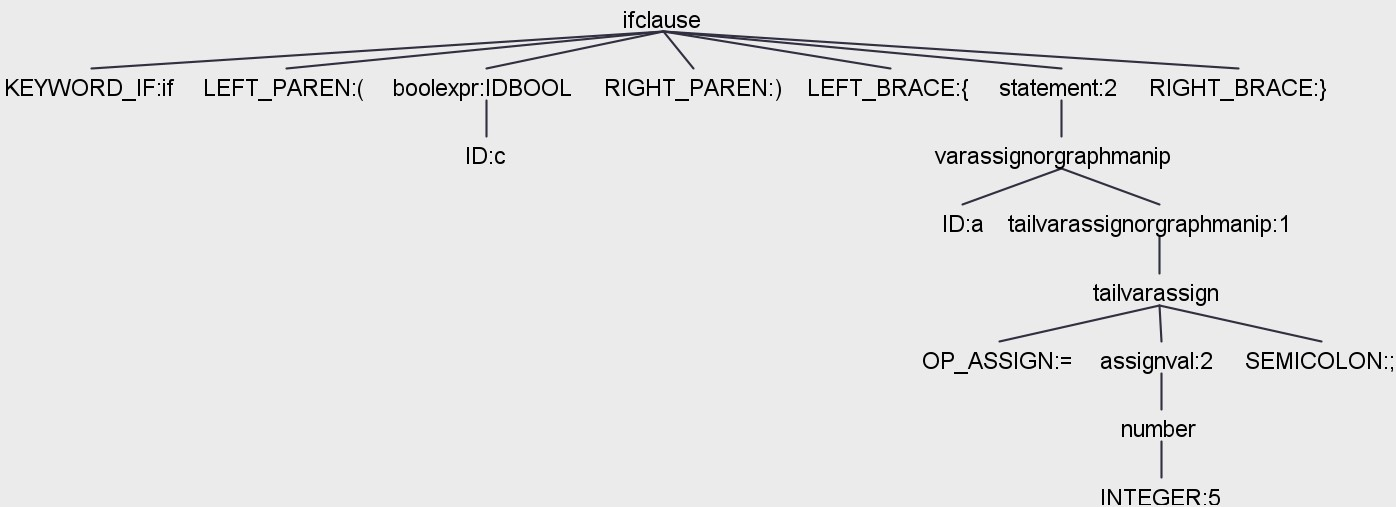
\includegraphics[height = 5cm]{figures/parse_trees/parseTree_ifClause}
    \caption{Parse tree for the if clause in the following if statement : \texttt{if(c)\{
    a = 5;\}
    else \{
    b = 3;\}}}
    \label{fig:parseTree_ifClause}
\end{figure}

\begin{figure}[H]
    \centering
    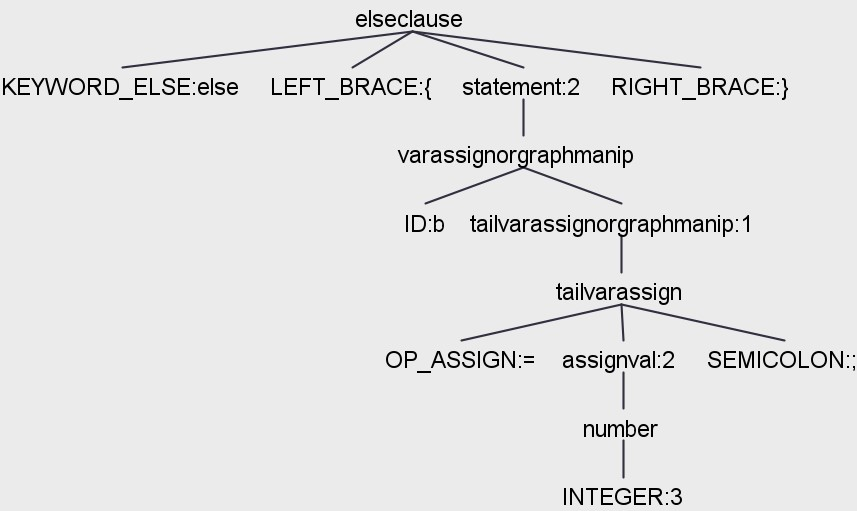
\includegraphics[height = 5cm]{figures/parse_trees/parseTree_elseClause}
    \caption{Parse tree for the else clause in the following if statement : \texttt{if(c)\{
    a = 5;\}
    else \{
    b = 3;\}}}
    \label{fig:parseTree_elseClause}
\end{figure}

\subsubsection*{While loop}

The statement starts with the keyword \texttt{while} followed by the condition for the loop and then the block of code to repeat.

\begin{align*}
\mathit{WhileBlock} &\rightarrow \text{keywordWhile} \: \text{leftParen} \: \mathit{BoolExpr} \: \text{rightParen} \: \text{leftBrace} \: \{ \mathit{statement}\} \: \text{rightBrace}
\end{align*}
\captionedgrammar{Description of a while loop}

\begin{figure}[H]
    \centering
    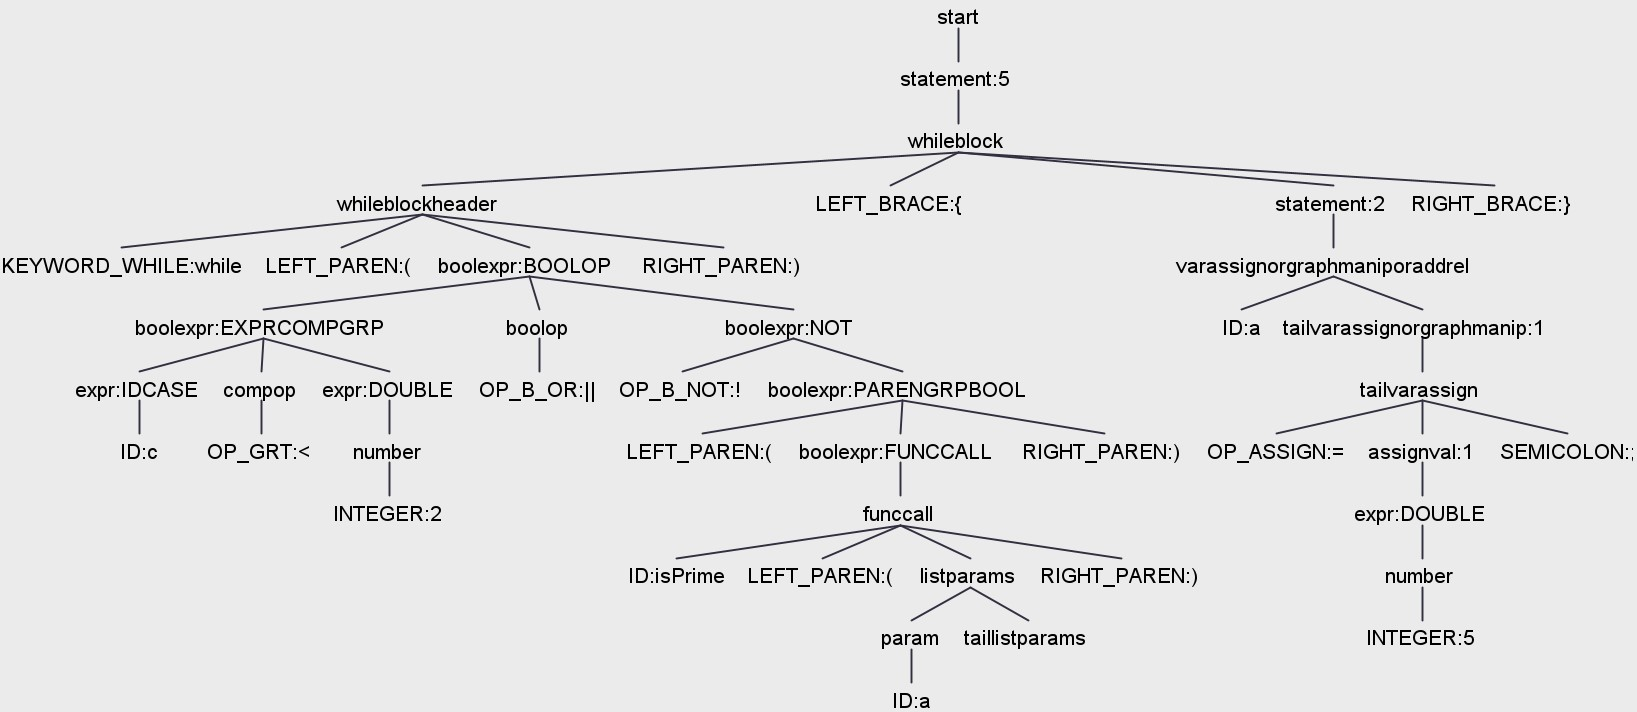
\includegraphics[height = 5cm]{figures/parse_trees/parseTree_whileblock}
    \caption{Parse tree for the following while statement with a more complex boolean expression that includes a function call : \texttt{while(c < 2 || !(isPrime(a)))\{
        a = 5;\}}}
    \label{fig:parseTree_whileblock}
\end{figure}

\subsubsection*{Function definition and function call}

Function definitions are introduced with the keyword $\texttt{def}$, followed by the name of the function, the types and names of the arguments and then the block of code executed by the function.
The keyword $\texttt{def}$ allows to distinguish the function declaration from a variable declaration because otherwise both statements would start with a type token.
It is possible to have a rule for both statements, as with the $\mathit{VarAssignOrGraphManip}$ rule, but that would mean that function declaration has the same rules as any statement and we couldn't use the grammar to enforce that function declaration can't be done in a $\texttt{while}$ or $\texttt{if-else}$ block of code.\\

A return statement is necessary to write a function so there is a rule describing it.
However, the parser can't enforce that necessity to have a return statement in a function, because it could be written in an $\texttt{if-else}$ block of code which makes it indistinguishable from standard statement.

Once defined, the function can then be called in the contexts mentioned above, by writing the function name and the parameters.

\begin{align*}
    \omit $\mathit{FuncDef}$ \hfil &\rightarrow \text{keywordDef} \: \mathit{Type} \: \text{varID leftParen} [\mathit{ListArgs}] \text{rightParen} \\
    & \text{leftBrace} \: \{ \mathit{statement} \} \: \text{rightBrace} \\
    \omit $\mathit{ListArgs}$ \hfil &\rightarrow \mathit{Arg} \:  \mathit{TailListArgs} \\
    \omit $\mathit{Arg}$ \hfil &\rightarrow \mathit{Type} \: \text{varId} \\
    \omit $\mathit{TailListArgs}$ \hfil & \rightarrow \{ \text{comma} \: \mathit{Arg} \} \\
    \omit $\mathit{ReturnStatement}$ \hfil &\rightarrow \text{keywordReturn} \: \mathit{AssignVal} \: \text{semicolon} \\
    \omit $\mathit{FuncCall}$ \hfil &\rightarrow \: \text{varID leftParen} [\mathit{ListParam}] \: \text{rightParen} \\
    \omit $\mathit{ListParam}$ \hfil &\rightarrow \mathit{varID} \:  \{ \text{comma} \: \mathit{varID} \}
\end{align*}
\captionedgrammar{Rules for function definitions and function calls}

\begin{figure}[H]
    \centering
    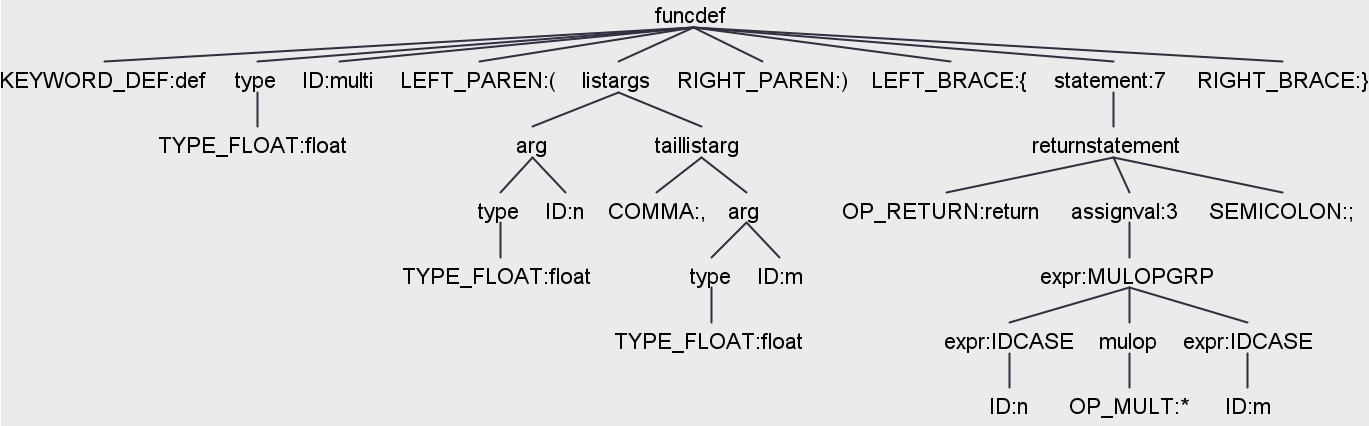
\includegraphics[height = 5cm]{figures/parse_trees/parseTree_funcdef}
    \caption{Parse tree for the following function definition : \texttt{def float multi(float n, float m)\{return n*m;\}} }
    \label{fig:parseTree_funcdef}
\end{figure}

